\documentclass{article}
\usepackage[margin=1in]{geometry}
\usepackage{graphicx}
\usepackage{caption}
\usepackage{subcaption}
\usepackage{amsmath}
\usepackage{amssymb}
\usepackage{booktabs}
\usepackage{color}
\usepackage{xcolor}
\usepackage{hyperref}

\title{Emotion Recognition}
\author{Arashdeep Mehroke \and Mohamed Hasan}
\date{Dec 5, 2024}
\begin{document}
\maketitle
%%%%%%%%%%%%%%%%%%%%%%%%%%%%%%%%%%%%%%%%%%%%%%%%%%%%%%%%%%%%%%%%%%%%%%%%%%%%%%%%%%%%%%%%%%%%%%%%%%%%%%%%%%%%%%
\section{Problem Statement}

Recognizing human emotions is an essential aspect of understanding and improving human-computer interaction, 
providing insights into behavioral analysis, mental health monitoring, and customer experience optimization. 
The \textbf{Ryerson Audio-Visual Database of Emotional Speech and Song (RAVDESS)} offers a rich collection of 
labeled audio data that can be leveraged to develop robust machine learning models for emotion classification.

Despite the availability of advanced feature extraction techniques such as YAMNet embeddings and Librosa-based 
handcrafted features, achieving high accuracy in emotion recognition remains a challenge due to:
\begin{enumerate}
    \item \textbf{High Dimensionality of Features:} Audio features like YAMNet embeddings are inherently high-dimensional, 
    complicating the training process for traditional models.
    \item \textbf{Imbalanced Datasets:} Emotional classes often exhibit uneven distributions, leading to biased model 
    performance.
    \item \textbf{Complexity of Audio Signals:} Variations in pitch, tone, and intensity across speakers make it difficult 
    to accurately classify emotions.
    \item \textbf{Computational Overheads:} Extracting, visualizing, and analyzing audio features for large datasets 
    requires efficient preprocessing and dimensionality reduction.
\end{enumerate}

This project aims to address these challenges by:
\begin{enumerate}
    \item Employing state-of-the-art feature extraction techniques (e.g., YAMNet, Librosa).
    \item Balancing the dataset using synthetic techniques like SMOTE.
    \item Experimenting with various machine learning and deep learning models to identify optimal solutions.
    \item Visualizing high-dimensional feature spaces with dimensionality reduction tools like t-SNE and UMAP for 
    better interpretability.
\end{enumerate}

The goal is to build a robust, scalable system capable of accurately classifying human emotions across multiple 
categories while ensuring computational efficiency and practical applicability.

%%%%%%%%%%%%%%%%%%%%%%%%%%%%%%%%%%%%%%%%%%%%%%%%%%%%%%%%%%%%%%%%%%%%%%%%%%%%%%%%%%%%%%%%%%%%%%%%%%%%%%%%%%%%%%
\section{Data Source}

The dataset used in this project is the \textbf{Ryerson Audio-Visual Database of Emotional Speech and Song (RAVDESS)}. 
It consists of 1440 audio files (16-bit, 48kHz \texttt{.wav}) featuring 24 professional actors (12 female, 12 male) 
vocalizing two statements in a neutral North American accent. 

\subsection{Emotions and Features}
The dataset includes 8 emotions: neutral, calm, happy, sad, angry, fearful, surprised, and disgusted, with normal and 
strong intensities (except neutral). Each statement is repeated twice, resulting in 60 trials per actor.

\subsection{Filename Structure}
Files are named using a 7-part numerical identifier (e.g., \texttt{03-01-06-01-02-01-12.wav}) indicating:
\begin{itemize}
    \item \textbf{Modality:} Audio-only (03).
    \item \textbf{Vocal Channel:} Speech (01).
    \item \textbf{Emotion:} Fearful (06).
    \item \textbf{Intensity:} Normal (01).
    \item \textbf{Statement:} Dogs (02).
    \item \textbf{Repetition:} First (01).
    \item \textbf{Actor:} Actor 12 (female).
\end{itemize}

%%%%%%%%%%%%%%%%%%%%%%%%%%%%%%%%%%%%%%%%%%%%%%%%%%%%%%%%%%%%%%%%%%%%%%%%%%%%%%%%%%%%%%%%%%%%%%%%%%%%%%%%%%%%%%
\section{Methodology}

\subsection{Data Preprocessing}
This study uses audio datasets derived from the RAVDESS dataset, which include features extracted using Librosa 
and YAMNet libraries. Below is a summary of the datasets used:

\begin{itemize}
    \item \textbf{librosa\_balanced.csv:} 45 features, 7119 samples.
    \item \textbf{librosa\_extracted\_features.csv:} 45 features, 6439 samples.
    \item \textbf{yamnet\_balanced.csv:} 1025 features, 7119 samples.
    \item \textbf{yamnet\_extracted\_features.csv:} 1025 features, 6440 samples.
\end{itemize}

\subsubsection*{Feature Exploration}

Figure \ref{fig:label_distribution} illustrates the distribution of labels in the dataset. Most emotion classes 
are balanced, but the classes "Neutral" and "Surprise" are underrepresented. For this reason, Synthetic Minority 
Oversampling Technique (SMOTE) is used to address class imbalances.

\begin{figure}[!h]
    \centering
    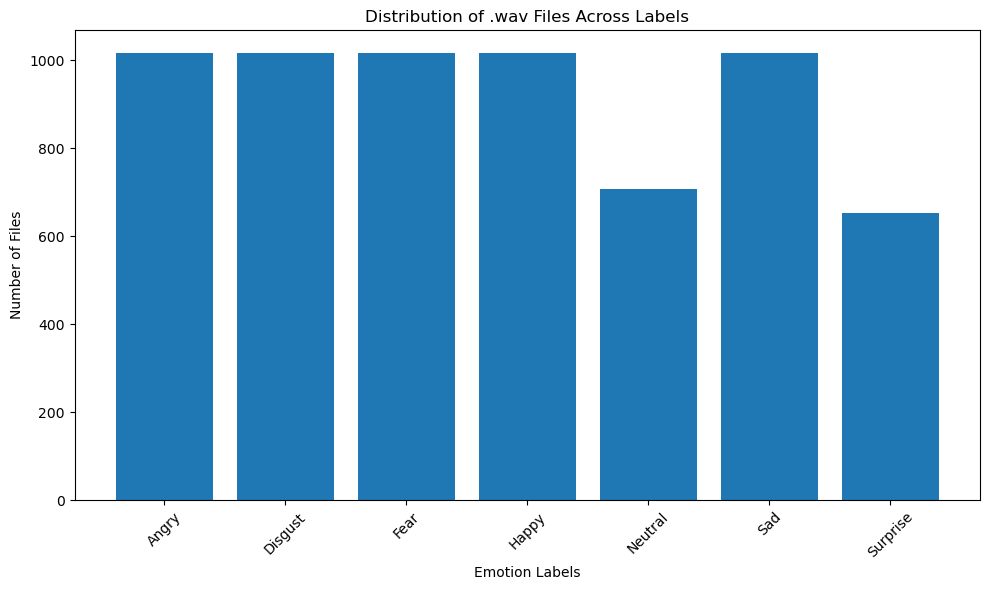
\includegraphics[width=0.7\textwidth]{../assets/label_distribution.png}
    \caption{Distribution of emotion labels across audio samples.}
    \label{fig:label_distribution}
\end{figure}

Feature distributions across the dataset were analyzed. Figure \ref{fig:feature_distributions} illustrates the 
distributions of key extracted features. The distributions reveal a variety of patterns in audio characteristics, 
which are useful for differentiating emotions.

\begin{figure}[!h]
    \centering
    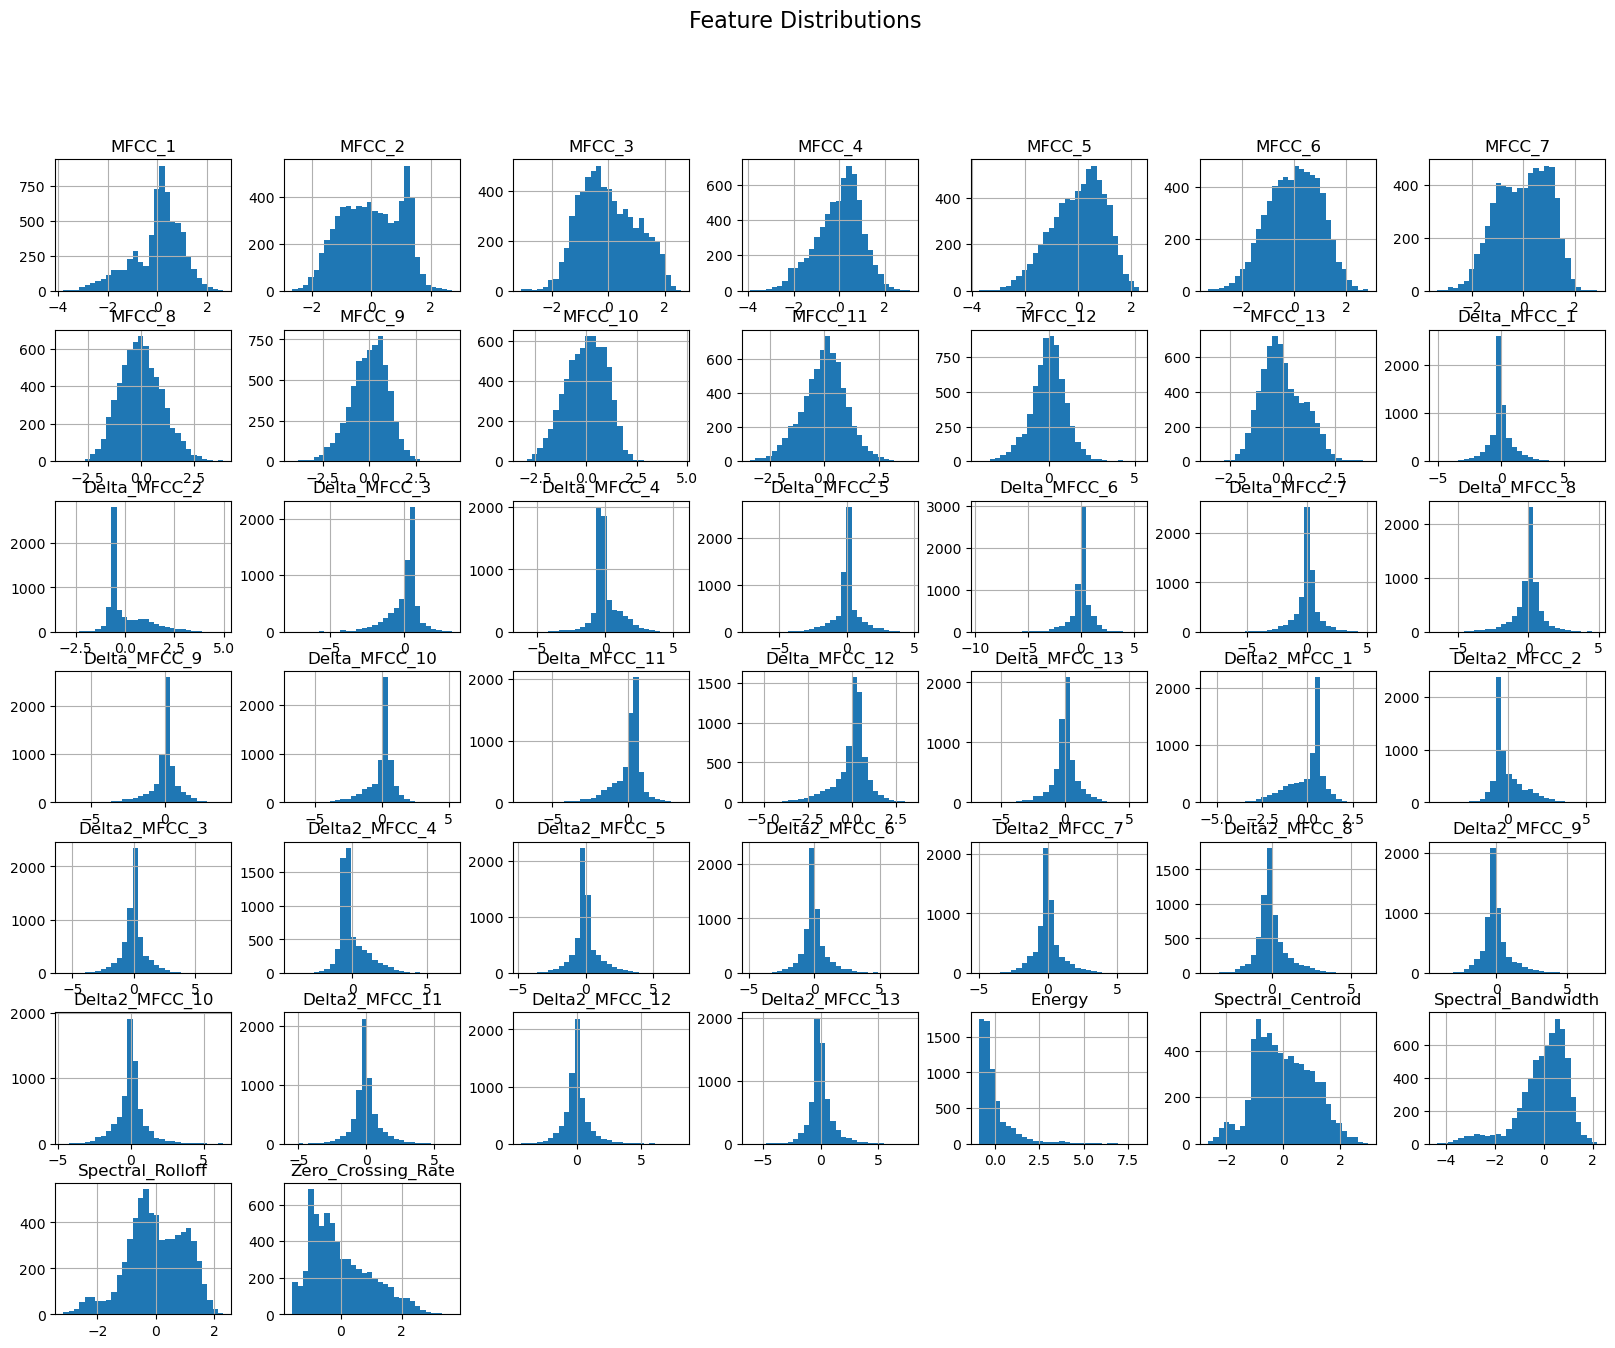
\includegraphics[width=0.8\textwidth]{../assets/feature_distributions.png}
    \caption{Feature distributions for extracted audio features, including MFCCs, spectral centroid, zero-crossing rate, 
    and energy.}
    \label{fig:feature_distributions}
\end{figure}

\subsubsection*{Feature Analysis}

Figures \ref{fig:mfcc_analysis} and \ref{fig:feature_variability} provide insights into the feature distributions and 
variability for the extracted features.

\begin{itemize}
    \item \textbf{MFCCs:} The Mel-Frequency Cepstral Coefficients (MFCCs) capture timbral information. Peaks and valleys 
    in the MFCC values are indicative of variations in speech timbre across emotions.
    \item \textbf{Spectral Centroid:} Represents the "brightness" of the audio. High centroid values suggest a higher 
    frequency content, while lower values are linked to softer tones.
    \item \textbf{Zero-Crossing Rate (ZCR):} Indicates the noisiness or percussiveness of the signal. Higher ZCR values 
    correspond to noisier audio signals, such as the "Surprise" class.
    \item \textbf{Energy:} Captures the loudness or intensity of the audio signal. Emotions like "Angry" and "Happy" show 
    higher energy levels compared to "Sad" and "Neutral."
\end{itemize}

\begin{figure}[!h]
    \centering
    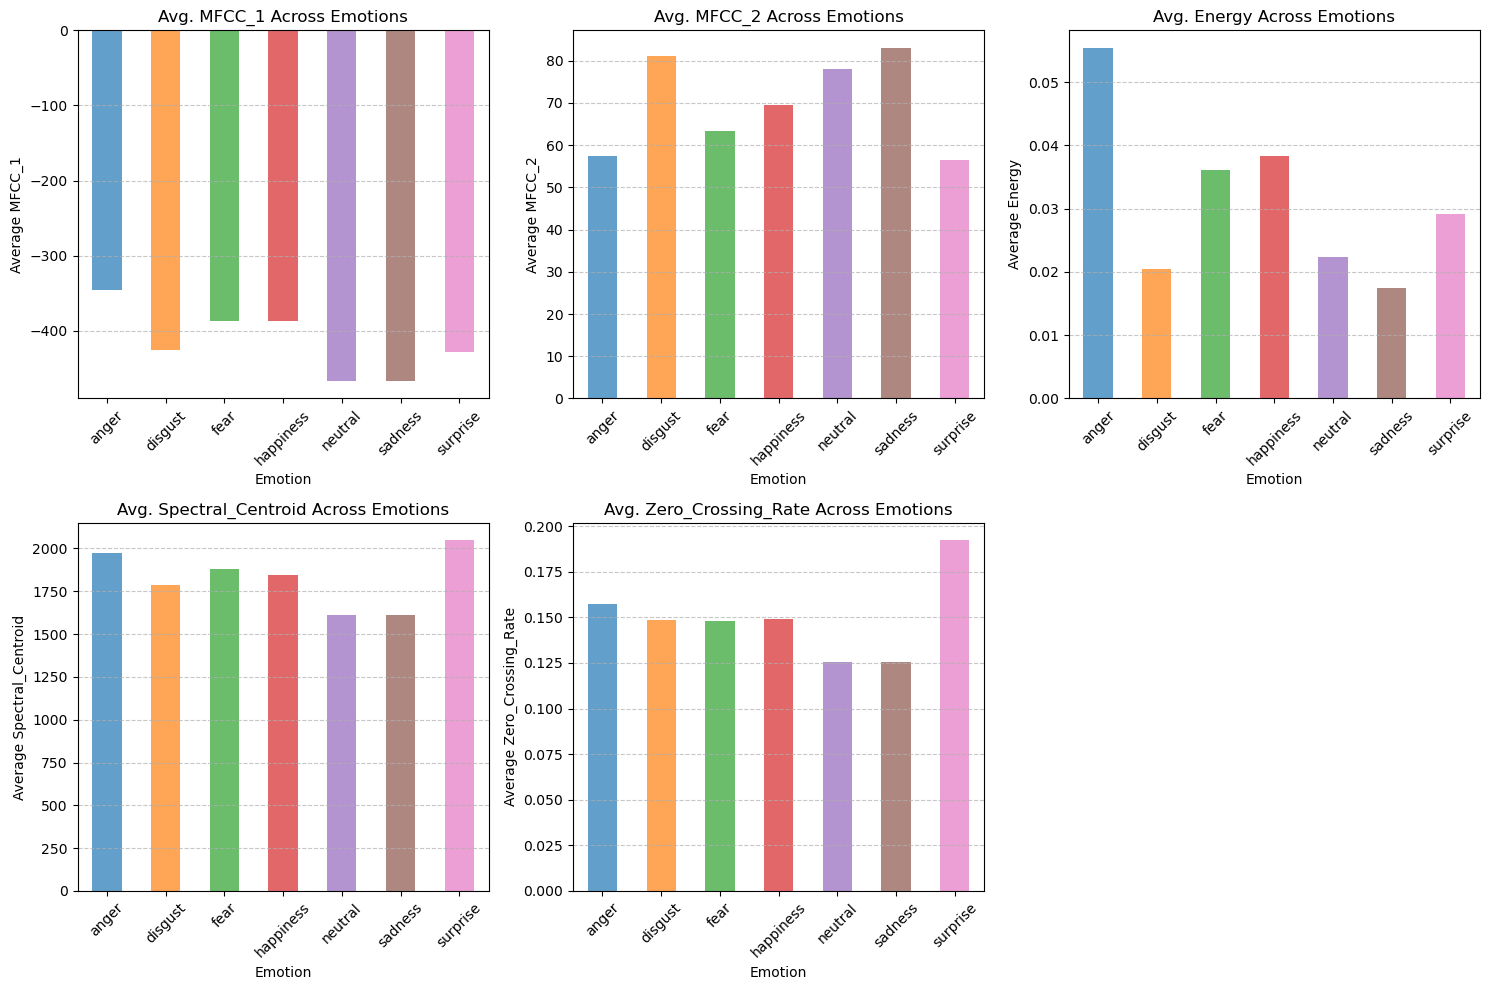
\includegraphics[width=0.8\textwidth]{../assets/mfcc_analysis.png}
    \caption{Mean values of MFCCs, Spectral Centroid, Zero-Crossing Rate, and Energy across emotions.}
    \label{fig:mfcc_analysis}
\end{figure}

\begin{figure}[!h]
    \centering
    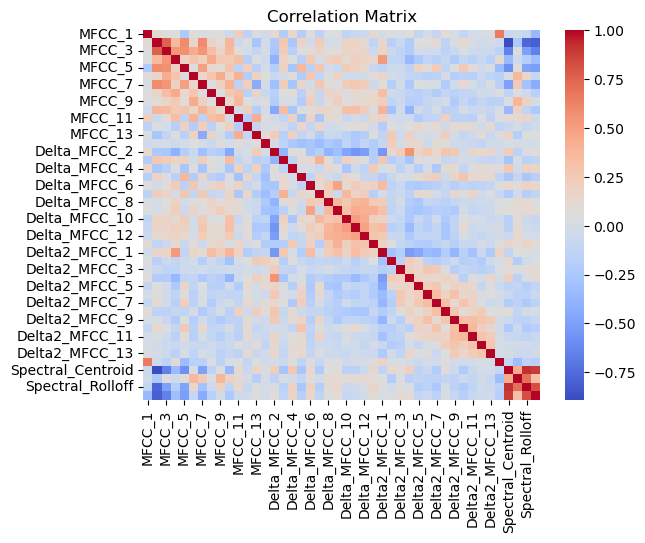
\includegraphics[width=0.8\textwidth]{../assets/feature_variability.png}
    \caption{Distribution of feature values across all extracted features.}
    \label{fig:feature_variability}
\end{figure}

\subsubsection*{Dimensionality Reduction}

Dimensionality reduction techniques such as PCA and t-SNE were applied to visualize the feature space. 
Figure \ref{fig:pca_visualization} demonstrates clustering of the dataset using PCA. Despite overlapping clusters, 
PCA highlights trends in feature separability.

\begin{figure}[!h]
    \centering
    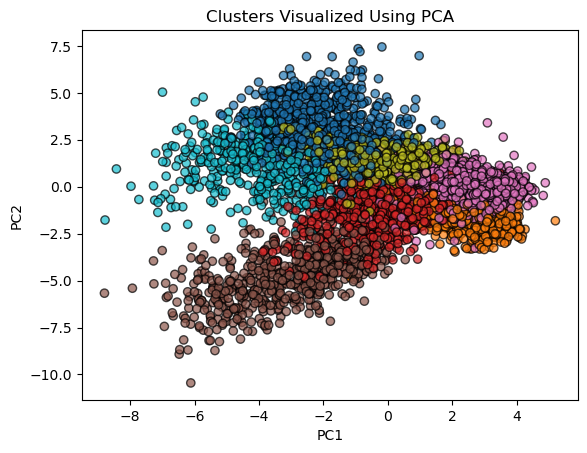
\includegraphics[width=0.6\textwidth]{../assets/pca_visualization.png}
    \caption{Clusters visualized using PCA. The clustering indicates some separation between emotion classes, 
    though significant overlap is observed.}
    \label{fig:pca_visualization}
\end{figure}

To address class imbalances, SMOTE (Synthetic Minority Oversampling Technique) was applied, and t-SNE was used to 
assess the improved separability of the dataset. Figure \ref{fig:tsne_visualization} highlights how t-SNE captures 
the non-linear relationships among features, improving the clustering of emotions.

\begin{figure}[!h]
    \centering
    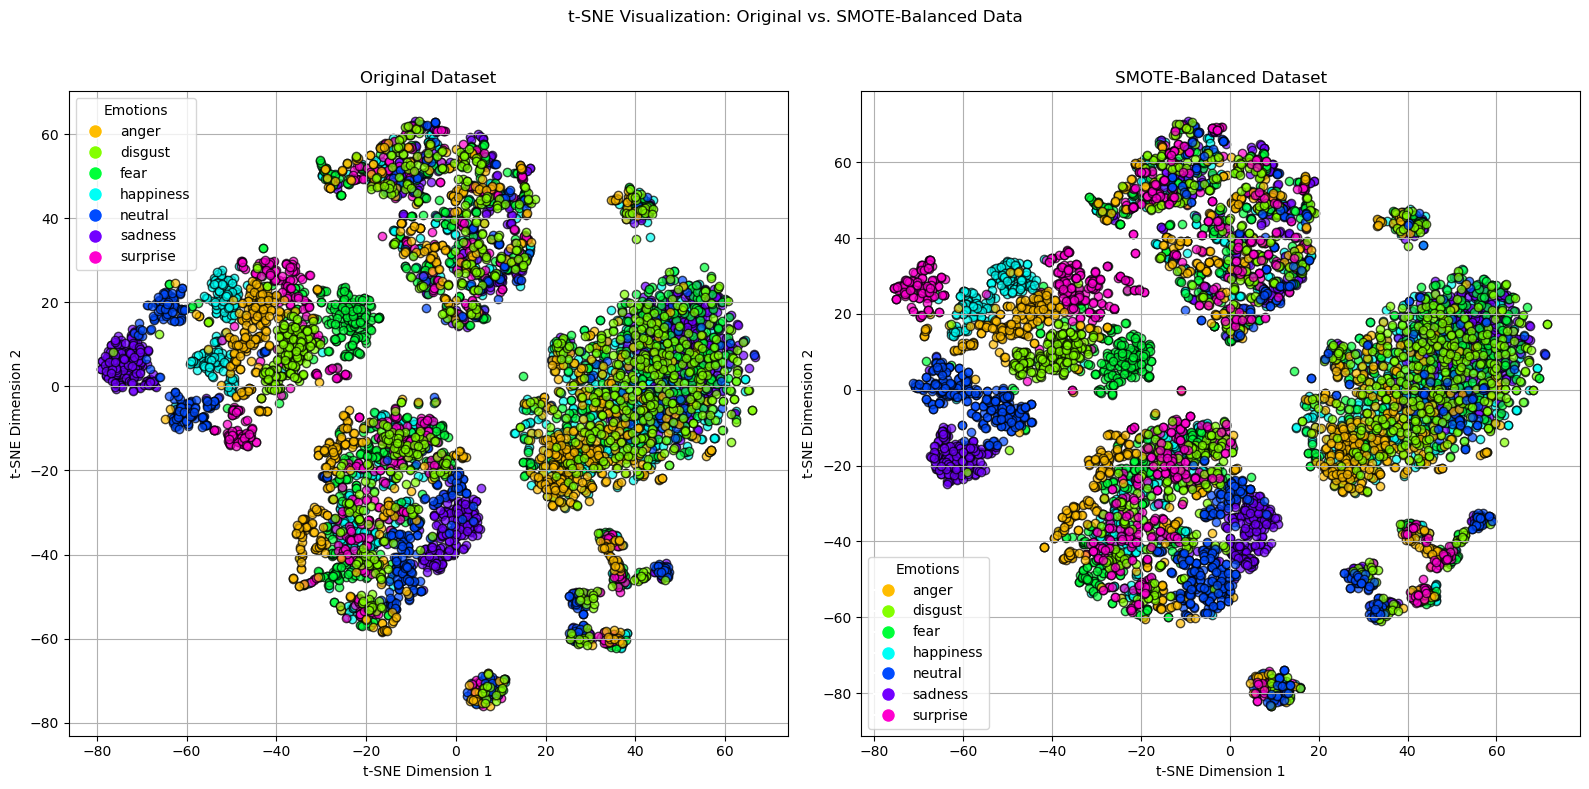
\includegraphics[width=0.8\textwidth]{../assets/tsne_visualization.png}
    \caption{t-SNE visualization of original and SMOTE-balanced datasets. Non-linear feature relationships are 
    effectively captured, enabling better emotion classification.}
    \label{fig:tsne_visualization}
\end{figure}

%%%%%%%%%%%%%%%%%%%%%%%%%%%%%%%%%%%%%%%%%%%%%%%%%%%%%%%%%%%%%%%%%%%%%%%%%%%%%%%%%%%%%%%%%%%%%%%%%%%%%%%%%%%%%%

\subsubsection*{Model Selection}
To classify emotions from the extracted audio features, four machine learning models were employed: K-Nearest Neighbors 
(KNN), Support Vector Machine (SVC), Random Forest, and a Multi-Layer Perceptron (MLP). Grid search was used to optimize 
the hyperparameters for KNN, SVC, and Random Forest, while MLP was manually tuned to align with the complexity of the problem.

\begin{itemize}
    \item \textbf{K-Nearest Neighbors (KNN):} 
    KNN was chosen for its simplicity and interpretability. It performs well in scenarios where emotion classes have 
    non-linear boundaries, as it classifies based on the proximity of similar feature patterns. KNN serves as an 
    effective baseline for understanding how well the extracted features group emotions in the feature space.

    \item \textbf{Support Vector Machine (SVC):} 
    SVC is particularly suited for high-dimensional datasets like YAMNet features, as it seeks to find the optimal 
    margin between classes. Its ability to use kernel functions allows it to capture both linear and non-linear decision 
    boundaries, making it a strong candidate for emotion classification where subtle differences in feature values 
    distinguish emotions such as "Happy" and "Fearful."

    \item \textbf{Random Forest:} 
    Random Forest was selected for its robustness and ability to handle heterogeneous data, such as a mix of spectral 
    and temporal features. It combines decision trees to handle complex interactions among features, which is crucial in 
    capturing the intricate variations in speech and audio characteristics associated with different emotions.

    \item \textbf{Multi-Layer Perceptron (MLP):} 
    MLP was chosen for its ability to model complex, non-linear relationships in the data. Emotions often involve subtle, 
    overlapping patterns in features like energy, spectral centroid, and MFCCs, which MLP can effectively learn. Its 
    hierarchical feature learning capability makes it particularly well-suited for tasks like emotion recognition, though 
    it requires careful tuning to prevent overfitting.
\end{itemize}

\subsubsection*{Hyperparameter Tuning}

Grid search was applied to systematically explore the hyperparameter space for KNN, SVC, and Random Forest. For KNN, the 
number of neighbors and distance metrics were tuned; for SVC, the kernel type, regularization parameter (\textit{C}), and 
kernel coefficient (\textit{gamma}) were optimized; and for Random Forest, the number of trees (\textit{n\_estimators}), 
maximum tree depth (\textit{max\_depth}), and minimum samples per split (\textit{min\_samples\_split}) were adjusted. 
MLP was tuned manually based on its learning rate, number of hidden layers, and neurons per layer.

\subsubsection*{Model Evaluation}

All models were evaluated using metrics relevant to the emotion classification task: accuracy, precision, recall, and 
F1-score. These metrics were chosen to balance the trade-offs between false positives and false negatives, which are critical 
for applications like affective computing. Cross-validation was employed to ensure robust evaluation, particularly given the 
imbalanced nature of certain emotion classes. The results of these evaluations are discussed in detail in the subsequent sections.








%%%%%%%%%%%%%%%%%%%%%%%%%%%%%%%%%%%%%%%%%%%%%%%%%%%%%%%%%%%%%%%%%%%%%%%%%%%%%%%%%%%%%%%%%%%%%%%%%%%%%%%%%%%%%%
\section*{Evaluation and Final Results}

The performance of the selected models (KNN, SVC, Random Forest, and MLP) was evaluated on multiple datasets using accuracy, 
precision, recall, and F1-score as metrics. The results are summarized in Table \ref{tab:results_summary} and visualized in 
Figures \ref{fig:accuracy_plot} and \ref{fig:other_metrics_plot}.

\subsubsection*{Summary of Results}

Table \ref{tab:results_summary} shows the performance metrics of all models across the different datasets. Accuracy is 
presented in a standalone graph (Figure \ref{fig:accuracy_plot}) to emphasize its importance in emotion classification 
tasks, while precision, recall, and F1-score are grouped together in Figure \ref{fig:other_metrics_plot} for a 
comprehensive comparison.

\begin{table}[h!]
\centering
\caption{Performance Summary of Models Across Datasets}
\label{tab:results_summary}
\begin{tabular}{|l|l|c|c|c|c|}
\hline
\textbf{Dataset} & \textbf{Model} & \textbf{Accuracy} & \textbf{Precision} & \textbf{Recall} & \textbf{F1-Score} \\ \hline
yamnet\_extracted\_features & MLPClassifier & 0.654 & 0.653 & 0.655 & 0.653 \\ \hline
yamnet\_balanced & MLPClassifier & 0.697 & 0.696 & 0.697 & 0.696 \\ \hline
yamnet\_balanced & RandomForestClassifier & 0.642 & 0.636 & 0.642 & 0.634 \\ \hline
yamnet\_extracted\_features & SVC & 0.680 & 0.679 & 0.680 & 0.679 \\ \hline
librosa\_extracted\_features & SVC & 0.679 & 0.679 & 0.679 & 0.678 \\ \hline
% Add more rows as necessary
\end{tabular}
\end{table}

\subsubsection*{Visual Analysis of Results}

The model accuracies are depicted in Figure \ref{fig:accuracy_plot}, highlighting that the \textit{MLPClassifier} 
consistently outperformed other models on most datasets. The \textit{RandomForestClassifier}, while robust, showed 
slightly lower accuracy compared to SVC and MLP. 

\begin{figure}[!h]
    \centering
    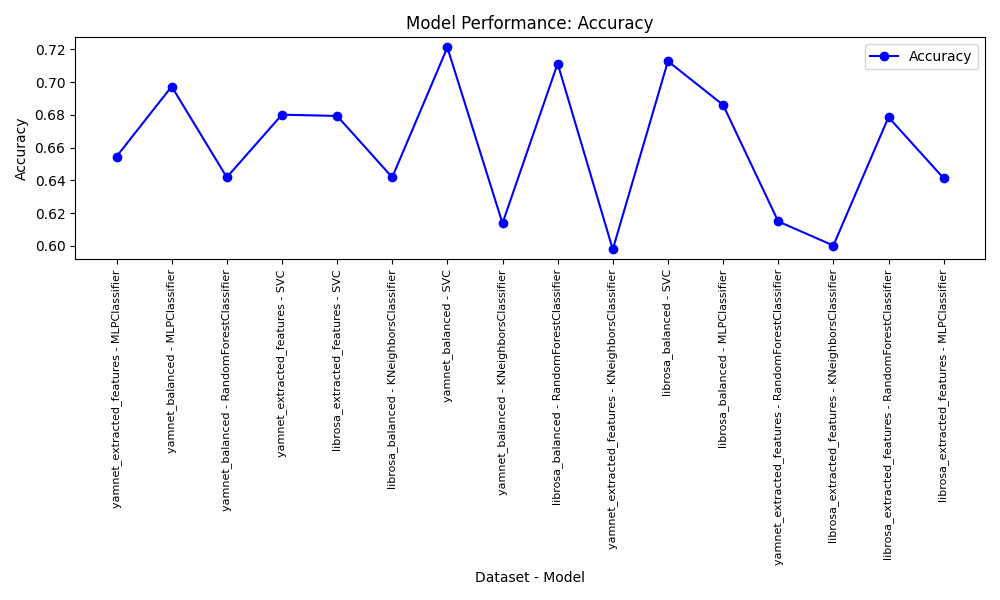
\includegraphics[width=0.8\textwidth]{../assets/model_performance_accuracy.png}
    \caption{Model Performance: Accuracy across datasets and models.}
    \label{fig:accuracy_plot}
\end{figure}

Precision, recall, and F1-score are shown in Figure \ref{fig:other_metrics_plot}. These metrics provide insights into 
how well the models balance false positives and false negatives, which is critical in emotion classification where 
misclassifications can have significant impact.

\begin{figure}[!h]
    \centering
    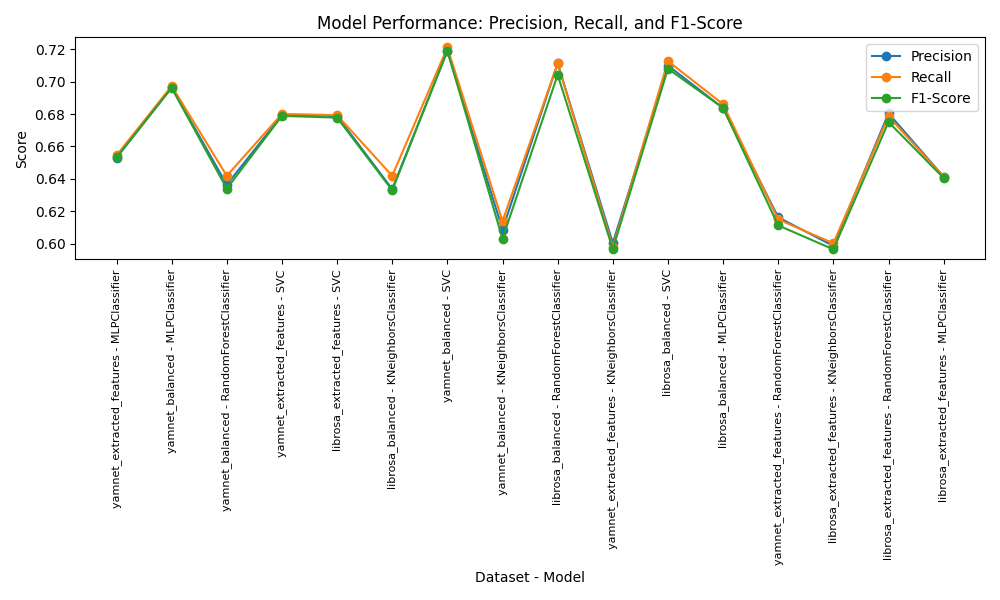
\includegraphics[width=0.8\textwidth]{../assets/model_performance_other_metrics.png}
    \caption{Model Performance: Precision, Recall, and F1-Score across datasets and models.}
    \label{fig:other_metrics_plot}
\end{figure}

%%%%%%%%%%%%%%%%%%%%%%%%%%%%%%%%%%%%%%%%%%%%%%%%%%%%%%%%%%%%%%%%%%%%%%%%%%%%%%%%%%%%%%%%%%%%%%%%%%%%%%%%%%%%%%

\section*{Conclusion}

The evaluation results highlight the strengths and limitations of the models tested for emotion classification 
based on extracted audio features. Audio classification, particularly emotion recognition, presents significant 
challenges due to the complex and overlapping nature of audio features, as well as the variability in how emotions 
are expressed across speakers and contexts. Key observations from this study include:

\begin{itemize}
    \item \textbf{SVC Achieved the Highest Accuracy:} 
    Across the datasets, \textit{Support Vector Classifier (SVC)} consistently delivered the highest accuracy, 
    showcasing its ability to handle high-dimensional feature spaces (e.g., YAMNet features) and complex decision 
    boundaries. The optimal hyperparameter tuning using grid search further contributed to its superior performance.

    \item \textbf{MLP Demonstrated Balanced Performance:} 
    The \textit{Multi-Layer Perceptron (MLP)} showed competitive performance, especially on the \textit{yamnet\_balanced} 
    dataset, where it achieved close to the highest scores across all metrics. MLP's ability to learn hierarchical 
    feature representations allowed it to handle the intricacies of audio features effectively. However, it requires 
    more careful tuning and computational resources to avoid overfitting.

    \item \textbf{Random Forest's Robustness:} 
    \textit{Random Forest} provided stable but slightly lower performance compared to SVC and MLP. Its robustness and 
    ability to handle heterogeneous data were evident, but it struggled with the subtle, high-dimensional relationships 
    present in audio features, which are critical for distinguishing nuanced emotional expressions.

    \item \textbf{KNN as a Baseline:} 
    \textit{K-Nearest Neighbors (KNN)} served as a baseline and performed reasonably well, demonstrating its simplicity 
    and effectiveness for non-linear feature spaces. However, its sensitivity to class imbalances and computational 
    inefficiency in high dimensions limited its overall performance.
\end{itemize}

\textbf{Challenges in Audio Emotion Classification:}
Emotion classification from audio data is inherently challenging due to:
\begin{itemize}
    \item \textbf{Feature Overlap:} Emotional states like "happy" and "surprise" or "sad" and "neutral" often share 
    overlapping spectral and temporal features, making them difficult to distinguish.
    \item \textbf{High Dimensionality:} Datasets such as those with YAMNet features contain hundreds of features, 
    necessitating robust models and hyperparameter optimization to avoid overfitting.
    \item \textbf{Class Imbalance:} Underrepresented classes like "surprise" require careful handling to ensure the 
    model does not favor dominant classes.
    \item \textbf{Speaker Variability:} Differences in tone, pitch, and accent across speakers can add noise to the 
    classification task, further complicating model training.
\end{itemize}

\textbf{Overall Findings:}
The results indicate that SVC is the most effective model for emotion classification in this study, particularly for 
high-dimensional datasets such as those with YAMNet features. Its ability to generalize across diverse datasets makes 
it an ideal choice for applications where precision and recall are critical. MLP demonstrated promising results and 
could benefit from further tuning and advanced architectures to potentially surpass SVC in future experiments.

\textbf{Future Work:}
To address the complexities of audio emotion classification, future efforts can focus on:
\begin{itemize}
    \item Advanced feature engineering and dimensionality reduction to improve feature quality and reduce computational complexity.
    \item Exploring deeper neural architectures or pre-trained audio models such as transformers for enhanced representation learning.
    \item Using ensemble methods to combine the strengths of SVC, MLP, and Random Forest for improved accuracy.
    \item Incorporating techniques such as domain adaptation to handle speaker variability and make models more robust.
\end{itemize}

This study highlights the critical importance of model selection and optimization in tackling the challenges of audio emotion 
classification, emphasizing the need for rigorous evaluation and future innovations in this domain.

%%%%%%%%%%%%%%%%%%%%%%%%%%%%%%%%%%%%%%%%%%%%%%%%%%%%%%%%%%%%%%%%%%%%%%%%%%%%%%%%%%%%%%%%%%%%%%%%%%%%%%%%%%%%%%
\section*{Citation}

\begin{quote}
Livingstone SR, Russo FA (2018). The Ryerson Audio-Visual Database of Emotional Speech and Song (RAVDESS). 
\textit{PLoS ONE}, 13(5): e0196391. \url{https://doi.org/10.1371/journal.pone.0196391}.
\end{quote}

For other uses, attribute as:  
\textit{"The RAVDESS by Livingstone \& Russo, licensed under CC BY-NA-SC 4.0."}


\end{document}